
\lecture{Confidence Intervals}{confidence-interval}
\section{Confidence Intervals}

\title{The Confidence Interval}
\subtitle{Introducing the Idea}

%\author{Kelly Black}
%\institute{Clarkson University}
\date{1 march 2013}

\begin{frame}
  \titlepage
\end{frame}

\begin{frame}
  \frametitle{Outline}
  \tableofcontents[pausesection,hideothersubsections,sectionstyle=show/hide]
\end{frame}


\subsection{Clicker Quiz}

\iftoggle{clicker}{%
  \begin{frame}
    \frametitle{Clicker Quiz}

    You sample a random variable which has a mean of 2.1 and a standard
    deviation of 4.5. You take 30 samples. What is the probability that
    the sample mean is more than 3.5?

    \vfill

    \begin{tabular}{l@{\hspace{3em}}l@{\hspace{3em}}l@{\hspace{3em}}l}
      A: 0.0446  & B: 0.6221  & C: 0.9954
    \end{tabular}

    \vfill
    \vfill
    \vfill

  \end{frame}
}

\subsection{The Confidence Interval}


\begin{frame}
  \frametitle{Problem!}

  We have a random variable. It has a mean, $\mu$, and a standard
  deviation, $\sigma$. How do we know?

  \vfill

  \only<2->
  {
    \begin{block}{Example}
      We run a capitol investment firm. Someone asks us for \$250,000
      to start a restaurant. It this a reasonable amount?
    \end{block}
  }

  \vfill

\end{frame}


\begin{frame}{The Big Question}

  How do we estimate the mean of a random variable?
  
\end{frame}


\begin{frame}{Example}
  
  We call up ten restaurant owners and ask them for the amount they
  needed to get started. We then calculate a \textit{sample mean},
  \begin{eqnarray*}
    \bar{x} & = & \frac{x_1 + x_2 + x_3 + x_4 + x_5 + x_6 + x_7 + x_8 + x_9 + x_{10}}{10}.
  \end{eqnarray*}
  This is our \textbf{estimate} for the mean.
  
\end{frame}


\iftoggle{clicker}{%
  \begin{frame}
    \frametitle{Clicker Quiz}

    We call up ten restaurant owners and ask them for the amount they
    needed to get started. We then calculate a \textit{sample mean},
    \begin{eqnarray*}
      \bar{x} & = & \frac{x_1 + x_2 + x_3 + x_4 + x_5 + x_6 + x_7 + x_8 + x_9 + x_{10}}{10}.
    \end{eqnarray*}

    Is this estimate close to the true mean?

    \vfill

    \begin{tabular}{l@{\hspace{3em}}l@{\hspace{3em}}l@{\hspace{3em}}l}
      A: Yes  & B: No  & C: Maybe??
    \end{tabular}

    \vfill
    \vfill
    \vfill

  \end{frame}
}


\begin{frame}{Estimators}

  The only thing that we have is $\bar{x}$ and $s$. The problem is
  that these things are random variables.

  $\bar{x}$ is an estimate for the mean, $\mu$.

  $s$ is an estimate for the standard deviation, $\sigma$.

  \begin{definition}{Bias}
    \begin{itemize}
    \item If our estimator for a parameter is expected to be less that
      the true value is has a \textit{negative bias.}
    \item If our estimator for a parameter is expected to be more that
      the true value is has a \textit{positive bias.}
    \item If the expectation of our estimator for a parameter is the
      same as the true value then it is \textit{unbiased.}
    \end{itemize}
  \end{definition}
  
  \vfill

\end{frame}

\begin{frame}{Estimator Of The Mean}

  \begin{definition}{Estimator of the mean}
    The sample mean is an estimator of the mean,
  \begin{eqnarray*}
    \bar{x} & = & \frac{x_1 + x_2 + x_3 + \cdots + x_{n}}{n}.
  \end{eqnarray*}    
  \end{definition}
  
  \vfill
  \vfill
  \vfill

\end{frame}


\begin{frame}{The Sample Mean}

\only<1>{\centerline{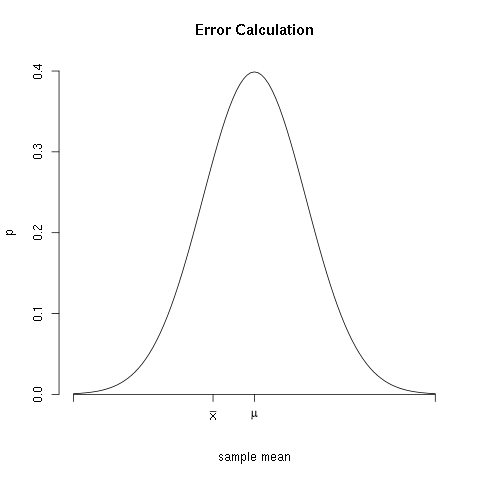
\includegraphics[width=6cm]{img/approximateMeanBlank}}}
\only<2>{\centerline{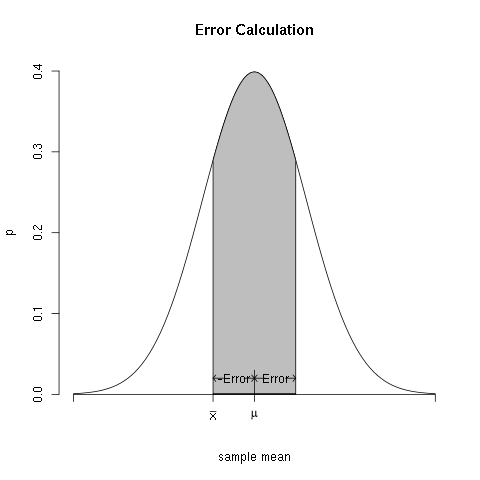
\includegraphics[width=6cm]{img/approximateMean}}}

Question: How close is $\bar{x}$ to $\mu$? 

Problem: We do not know what $\mu$ is!
  
\end{frame}


\begin{frame}{Confidence Interval}

  \begin{columns}
    \column{.4\textwidth}

    \centerline{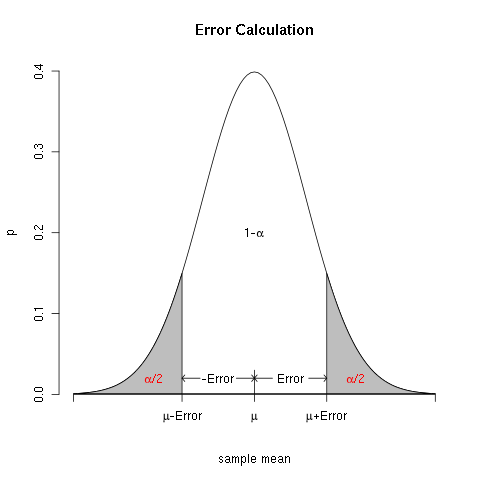
\includegraphics[width=4cm]{img/confidenceInterval}}

    \column{.6\textwidth}

    We want one of the following things:
    \begin{itemize}
    \item Determine the value of the error
    \item Determine number of samples (N)
    \item Determine the probability that we are outside of the error bounds.
    \end{itemize}

  \end{columns}
  
\end{frame}


\begin{frame}{Confidence Interval}

  \begin{columns}
    \column{.4\textwidth}
    \centerline{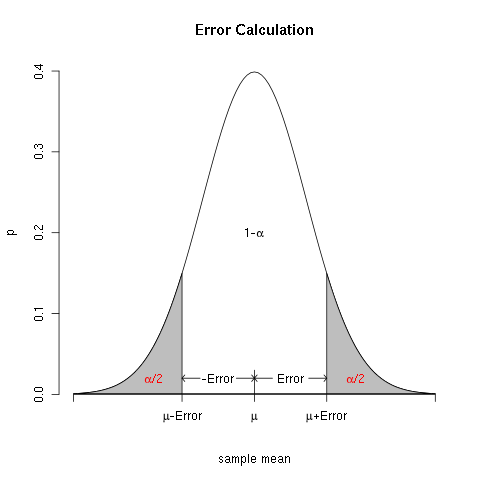
\includegraphics[width=4cm]{img/confidenceInterval}}

    \column{.6\textwidth}
    The key relationship:
    \begin{eqnarray*}
      p\lp \mu-\mathrm{error} \leq \bar{x} \leq \mu + \mathrm{error}\rp
      & = & 1-\alpha
    \end{eqnarray*}
    or
    \begin{eqnarray*}
      p\lp \bar{x} \leq \mu-\mathrm{error} \rp & = & \frac{\alpha}{2},
    \end{eqnarray*}
    and
    \begin{eqnarray*}
      z & = & \frac{-\mathrm{error}}{\sigma/n}.
    \end{eqnarray*}

  \end{columns}

\end{frame}



\iftoggle{clicker}{%
  \begin{frame}
    \frametitle{Clicker Quiz}


    \centerline{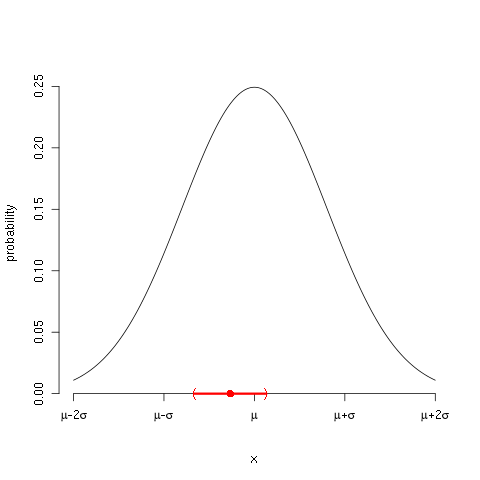
\includegraphics[width=6cm]{img/week8DistConfInterval}}
    If the value of $\alpha$ is increased does the length of the
    ``error'' increase or decrease?  \vfill

    \begin{tabular}{l@{\hspace{3em}}l@{\hspace{3em}}l@{\hspace{3em}}l}
      A: Increase  & B: Decrease
    \end{tabular}

    \vfill
    \vfill
    \vfill

  \end{frame}
}



\begin{frame}
  \frametitle{Estimator for the mean}


  \only<1>{\centerline{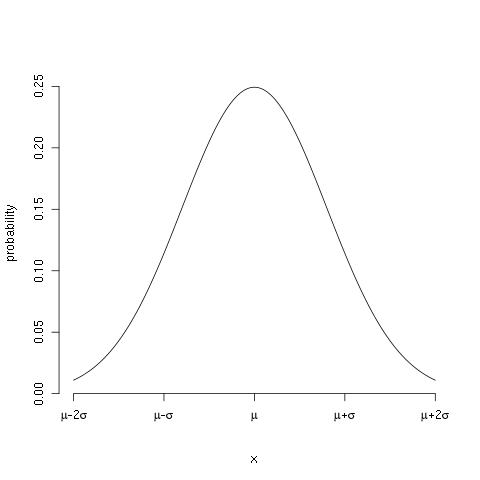
\includegraphics[width=6cm]{img/week8Dist}}}
  \only<2>{\centerline{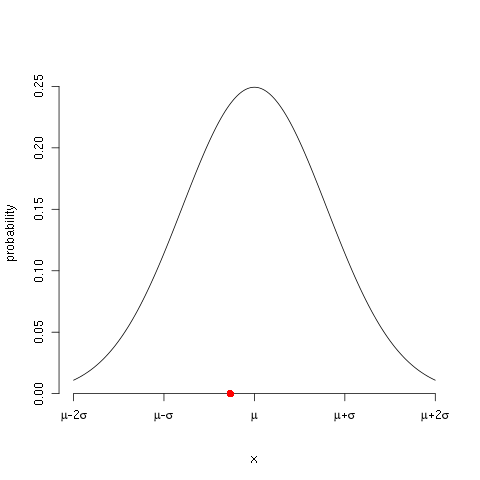
\includegraphics[width=6cm]{img/week8DistSample}}}
  \only<3>{%
    \centerline{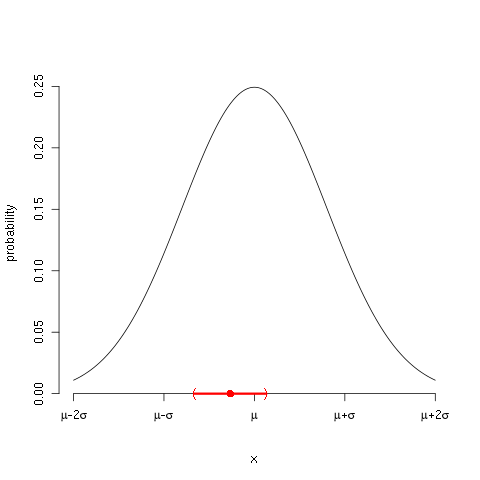
\includegraphics[width=6cm]{img/week8DistConfInterval}}

    We want to determine the probability that
    \begin{eqnarray*}
      \bar{x}-\mathrm{error} \leq \mu \leq \bar{x}+\mathrm{error}.
    \end{eqnarray*}

  }

\end{frame}

\begin{frame}{Confidence Interval}

  \begin{columns}
    \column{.4\textwidth}

    \centerline{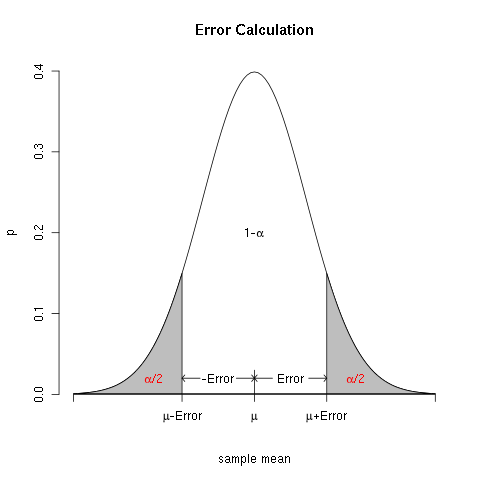
\includegraphics[width=4cm]{img/confidenceInterval}}

    \column{.6\textwidth}

    We want one of the following things:
    \begin{itemize}
    \item Given $N$ and $\alpha$ calculate the error
    \item Given $N$ and the error calculate $\alpha$
    \item Given $\alpha$ and the error calculate $N$
    \end{itemize}

  \end{columns}
  
\end{frame}


\begin{frame}{The Relationship Between $N$, error, and $\alpha$}

  \only<1-2>%
  {
    We want to determine the probability that
    \begin{eqnarray*}
      \bar{x}-\mathrm{error} \leq \mu \leq \bar{x}+\mathrm{error}.
    \end{eqnarray*}
    but we can work with the relationship
    \begin{eqnarray*}
      p\lp \mu-\mathrm{error} \leq \bar{x} \leq \mu + \mathrm{error}\rp
      & = & 1-\alpha      
    \end{eqnarray*}
  }

    Focus on the error term,
    \begin{eqnarray*}
      \mu-\mathrm{error} \leq \bar{x} \leq \mu + \mathrm{error} 
    \end{eqnarray*}
    \begin{eqnarray*}
      \only<2->%
      {
        \Rightarrow
      }
      \begin{array}{rcl@{\hspace{1.5em}\mathrm{and}\hspace{1.5em}}rcl}
        \only<2->%
        {
          \mu-\mathrm{error} & \leq & \bar{x} & \bar{x} & \leq & \mu + \mathrm{error} \\
        }
        \only<3->%
        {
          \mu & \leq & \bar{x}+\mathrm{error} & \bar{x}- \mathrm{error}  & \leq & \mu  \\
          \bar{x}+\mathrm{error} & \geq & \mu  & \mu & \geq & \bar{x}- \mathrm{error} \\
        }
      \end{array}
    \end{eqnarray*}
    \only<4->%
    {
      This implies that 
      \begin{eqnarray*}
        \bar{x}-\mathrm{error} \leq  \mu \leq \bar{x} + \mathrm{error} 
      \end{eqnarray*}
    }
  
\end{frame}


\begin{frame}{Life is good}
  We want to determine the probability that
  \begin{eqnarray*}
    \bar{x}-\mathrm{error} \leq \mu \leq \bar{x}+\mathrm{error}.
  \end{eqnarray*}
  but that is the same as working with the relationship
    \begin{eqnarray*}
      p\lp \mu-\mathrm{error} \leq \bar{x} \leq \mu + \mathrm{error}\rp
      & = & 1-\alpha.
    \end{eqnarray*}

\end{frame}

\begin{frame}{Simulation}

  See the simulation.
  
\end{frame}


\begin{frame}
  \frametitle{Example}

  We contact ten restaurant owners and ask what their starting costs
  were. We get a sample mean of \$235,000 and a standard deviation of
  \$45,000. Find the 95\% confidence interval.

  \vfill

  \only<2->%
  {

    The 95\% confidence interval is from 207,109\$ to 262,891\$
    assuming a normal distribution with a sample size of ten.

  }

  \vfill

\end{frame}


% LocalWords:  Clarkson pausesection hideallsubsections hideothersubsections
% LocalWords:  sectionstyle
